\RequirePackage{amsthm} %https://tex.stackexchange.com/questions/687324/unknown-theoremstyle-warning-with-springer-nature-template
\documentclass[sn-mathphys-num,icol]{sn-jnl}
%\documentclass[sn-mathphys-num,iicol]{jnl}

%\usepackage{sn-jnl.sty}
\usepackage[pscoord]{eso-pic}% The zero point of the coordinate systemis the lower left corner of the page (the default).

\usepackage[absolute,overlay]{textpos}
\usepackage[dvipsnames]{xcolor}
\usepackage{tikz}
\usepackage{graphicx}% \usepackage{multirow}% \usepackage{cuted}
\usepackage{amsmath,amssymb,amsfonts}%
\usepackage{amsthm}%
\usepackage{physics}
\usepackage[locale=US]{siunitx}
\usepackage{mathrsfs}%
\usepackage[title]{appendix}%
\usepackage{xcolor}%
\usepackage{textcomp}%
\usepackage{manyfoot}%
\usepackage{booktabs}%
\usepackage{algorithm}%
\usepackage{algorithmicx}%
\usepackage{algpseudocode}%
\usepackage{listings}%
\usepackage{newtxmath}%
\usepackage{yfonts}
\usepackage{braket}
\usepackage{dsfont}
\usepackage{subfig}
\usepackage[tiny]{titlesec}%
\usepackage[american]{babel}
\usepackage{cleveref}

\usetikzlibrary{arrows.meta, positioning, shapes.geometric, decorations.markings}

\theoremstyle{thmstyleone}
\newtheorem{theorem}{Theorem}
\newtheorem{proposition}[theorem]{Proposition}

\theoremstyle{thmstyletwo}
\newtheorem{remark}{Remark}

\theoremstyle{thmstylethree}
\newtheorem{definition}{Definition}

\raggedbottom

\newcommand{\td}{\text{d}}

\titleformat{\subsection}{}{\thesubsection}{1em}{\itshape}
\titleformat{\subsubsection}{}{\thesubsubsection}{1em}{\itshape}

\begin{document}

\title{E214: ATLAS}
\author*[1]{\fnm{Dhruv} \sur{Pisharody}}\email{}
\author*[1]{\fnm{Angelo} \sur{Brade}}\email{s72abrad@uni-bonn.de}
\affil*[1]{Rheinische Friedrich--Wilhelms--Universität, Bonn}
\maketitle
\section{Introduction}
For this laboratory course simulated Atlas data is analysed. Particles like the gluon or muon are identified through the graphical program Atlantis. For quantitativ analysis the detector is calibrated with the Z-Boson mass and then used to measure the W-Boson mass.
\subsection{ATLAS detector}
The Atlas (A Toroidal LHC ApparatuS) detector is located at CERN (European Organization for Nuclear Research) to detect products of proton-proton collisions done through the LHC (Large Hadron Collider) at \SI{14}{TeV}\cite{cern_org}.
It consists of four main areas, the tracking system, the ECAL, the HCAL and the muon chambers. The tracking system is placed in the inner detector, being the closest to the collision with \SI{3.3}{cm} from the beam line. There, four layers of silicon pixel detectors, one layer of silicon sensors and another layer of straws, made up of a gold plated tungsten wire surrounded by gas, get for a specific trajectory multiple hits through which the original trajectory can be reconstructed.\cite{cern_org} Because of an externally applied magnetic field, the trajectory is curved through the relativistic Lorentz force. This way the momentum of charged particles is measured. To measure the energy of the particles the ECAL and HCAL is introduced. The ECAL (Electromagnetic CALoremeter) is build with a material transmissive enough to let heavy particles like hadrons, muons or tauons pass, but so dense that electrons collide with the constituting atoms such that they emit bremsstrahlung. The photons produced by this, given a high enough energy, produce themself electron positron pairs. This forms a so-called electromagnetic shower, which deposits its charge in the ECAL. This charge is read out by anodes and corresponds to an energy in quantisations of the electron charge. Similarly this is done in the HCAL (Hadron CALorimeter), where the more heavy particles deposit their charge. Except, here no EM showers are formed, but jets through the hadronization of fast quarks and gluons. Lastly in the muon chamber, the muons are detected.\cite{bonn_physics601_atlas_2025} Their trajectory also curves, due to a second external magnetic field, which is orthogonal to the field of the inner detector. When viewing the whole detector in polar coordinates, where the z-axis is directed along the particle beam, the outer magnetic field of the muon chambers is oriented along the rotation with the $\phi$-angle and the inner magnetic field is oriented with the z-axis. A schematic illustration of the whole detector can be seen in \Cref{fig:atlas}.
\begin{figure}[h]
	\begin{center}
		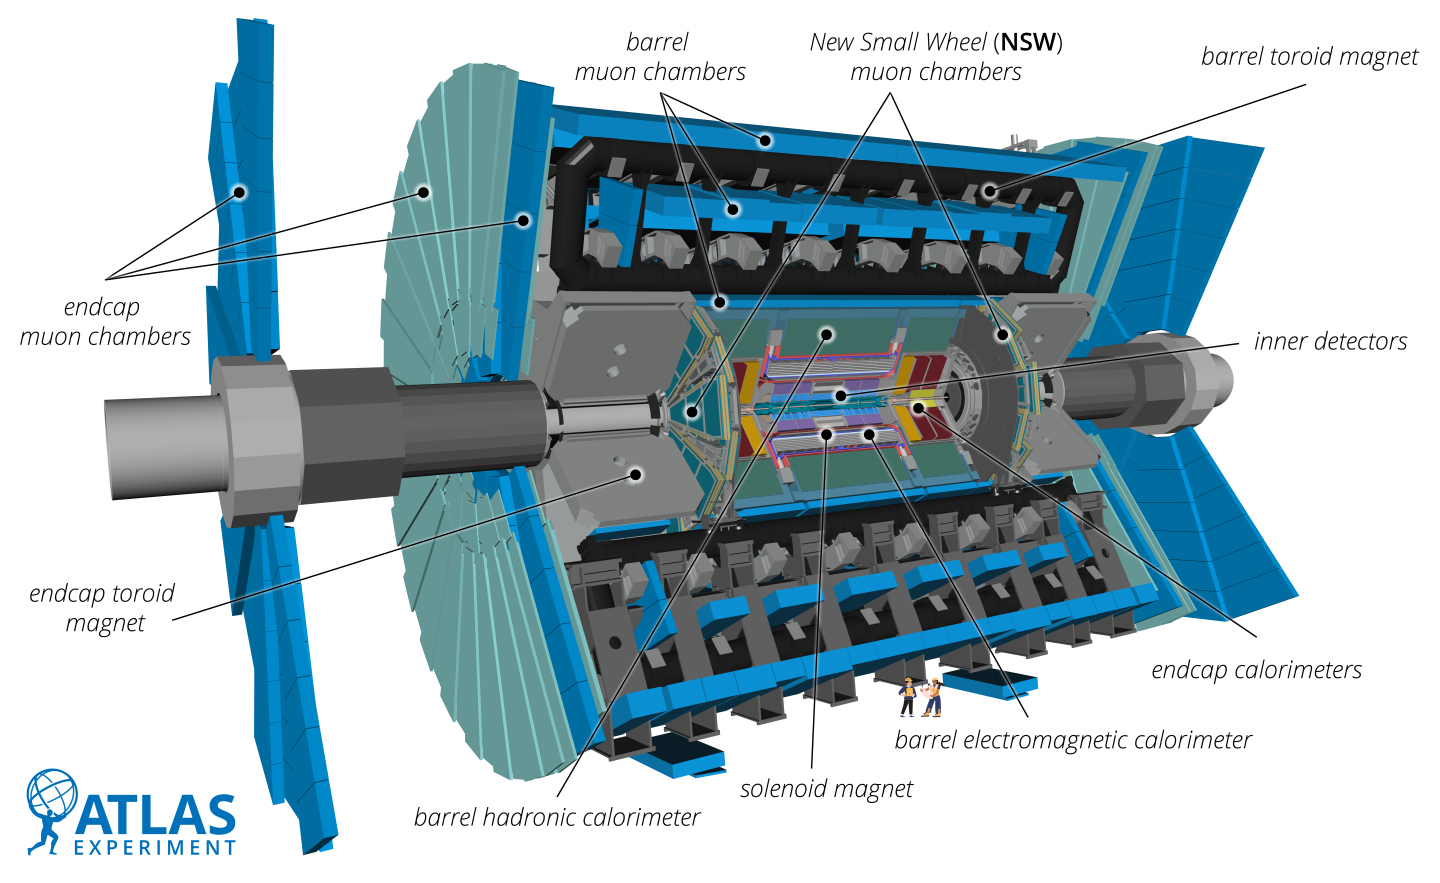
\includegraphics[width=1\textwidth]{../images/ATLAS-Experiment-Schematic-2022-Labels-People.png}
	\end{center}
	\caption{Schematic illustration of the ATLAS experiment, including new systems installed during Long Shutdown 2 (LS2).\cite{cern_org}}\label{fig:atlas}
\end{figure}
\section{Event Displays and Calibration}
The first task is to work with the graphical event display Atlantis, where different simulated events of the for an ATLAS detection are investigated. Furthermore the raw data needs to be calibrated with the well measured Z-Boson mass $m_Z$, though multiplicative scalar corrections of the energy for different angles $\theta$ and $\phi$. This is a good point to introduce the Lorentz invariant rapidity \[y=\frac{1}{2}\ln{\frac{E+p_z}{E-p_z}}\] Its usefulness gets apparent, when using the high energy approximation, where it gets reduced to the pseudo-rapidity \[\eta=-\ln{\tan{\frac{\theta}{2}}}\] Here it is seen that the non-Lorentz invariant angle $\theta$ can be replaced by the pseudo-rapidity, which will be Lorentz invariant for boosts along the z-axes. Together with the azimuthal angle $\phi$, the Lorentz invariant distance \[\Delta R = \sqrt{{\Delta\phi}^2+{\Delta\eta}^2}\] can be introduced.
\subsection{Questions to be answered before the lab}
\subsubsection{Decay of the $Z^0$ boson}
If a given $Z^0$ is at rest, the momentum of the electrons of the decay products $Z^0\rightarrow e^+ e^-$ are calculated through momentum and energy conservation. Using
\begin{align}
	0=\vec{p}_{Z^0}=\vec{p}_{e^+}+\vec{p}_{e^-} \Rightarrow |\vec{p}_{e^+}|=|\vec{p}_{e^-}|, \label{eq:mom} \\
	m_{e^+}=m_{e^-}\label{eq:mass}                                                                          \\
	\text{ and } E^2 = p^2+m^2\label{eq:energy}
\end{align}
the energy conservation \[E_{Z^0}=E_{e^+}+E_{e^-}\] can be rearranged to \[|\vec{p}_{e^-}|=\sqrt{\frac{m^2_{e^+}}{4}-m^2_{e^-}}\] Using $m_{Z^0}=\SI{91.1880+-0.0020}{GeV}$ and $m(e^-)=\SI{0.51099885069+-0.00000000016}{MeV}$, the momentum of the electron is \[|\vec{p}_{e^-}|=\SI{45.5940+-0.0010}{GeV}.\] Here, the electron mass and uncertainty could have been neglected.
\subsubsection{Scattering reaction $e^+e^-\rightarrow \tau^+\tau^-$}
In the center-of-mass system, given $\sqrt{s}=E_{\text{COM}}=\SI{5}{GeV}$ and
\begin{align}
	E_{\text{COM}}=E_{\tau^-}+E_{\tau^+},
\end{align}
\Crefrange{eq:mom}{eq:energy} can be used again to obtain
\begin{align}
	|\vec{p}_\tau| = \sqrt{\left(\frac{\sqrt{s}}{2}\right)^2-m^2_{\tau}}
\end{align}
For $m_{\tau}=\SI{1776.86+-0.12}{MeV}$ and no uncertainty on the center-of-mass energy, the momentum of the tauon is
\begin{align}
  |\vec{p}_{\tau}| = \SI{1.756+-0.068}{GeV}
\end{align}
\end{document}
